\documentclass{homeworg}
\usepackage{enumitem}
\usepackage{listings}
\usepackage{color} %red, green, blue, yellow, cyan, magenta, black, white
\definecolor{mygreen}{RGB}{28,172,0} % color values Red, Green, Blue
\definecolor{mylilas}{RGB}{170,55,241}
\usepackage{xcolor,cancel}
% --------------- GRAPHIC PACKAGES ----------------------------
\usepackage{graphicx}
\graphicspath{{./images/}}
\usepackage{wrapfig}
\newcommand\hcancel[2][black]{\setbox0=\hbox{$#2$}%
\rlap{\raisebox{.45\ht0}{\textcolor{#1}{\rule{\wd0}{1pt}}}}#2}

%\usepackage{authblk}
%\title{CSE 5301 - HW02}
%\author[1]{Bardia Mojra}
%\affil[1]{1000766739}
\begin{document}

% --------------- MATLAB Code settings -----------------------
\lstset{language=Matlab,%
    %basicstyle=\color{red},
    breaklines=true,%
    morekeywords={matlab2tikz},
    keywordstyle=\color{blue},%
    morekeywords=[2]{1}, keywordstyle=[2]{\color{black}},
    identifierstyle=\color{black},%
    stringstyle=\color{mylilas},
    commentstyle=\color{mygreen},%
    showstringspaces=false,%without this there will be a symbol in the places where there is a space
    numbers=left,%
    numberstyle={\tiny \color{black}},% size of the numbers
    numbersep=9pt, % this defines how far the numbers are from the text
    emph=[1]{for,end,break},emphstyle=[1]\color{red}, %some words to emphasise
    %emph=[2]{word1,word2}, emphstyle=[2]{style},
}

% --------------- Title -------------------------------------
%\maketitle
\begin{center}
\textbf{EE 5323 - HW04}\\
\end{center}

\noindent
Bardia Mojra\\
1000766739\\
\today\\
HW04 -- Vector Fields, Flows, First Integrals\\
EE 5323 -- Nonlinear Systems\\
Dr. Lewis

\exercise
\noindent
\textbf{First Integral of Motion for Undamped Oscillator}\\
\begin{equation*}
\ddot{x} + x = 0
\end{equation*}

\begin{enumerate}[label=(\alph*)]
  \item Write position-velocity state space form \(\dot{X} = f(X)\).
  \item Plot the trajectories \(x(t)\), \(\dot{x}(t)\) vs. time. Use initial conditions of \(x(0)=0.1\), \(\dot{x}(t)=0\).
  \item Plot the vector field \(f(X)\) in the phase plane \((x_1, x_2)=(x, \dot{x})\). Plot for points spaced in a uniform mesh in the box \(x_1=[-10,10]\), \(x_2=[-10,10]\).
  \item Plot the system trajectories (flows or orbits) in the phase plane. Take ICs spaced in a uniform mesh in the box \(x_1=[-10,10]\), \(x_2=[-10,10]\).
  \item Derive the First Integral of Motion \(F(x_1,x_2)\) as done in class. Plot the FIM as a 3-D surface over the phase plane on the \(x_1=[-10,10]\), \(x_2=[-10,10]\).
\end{enumerate}


\noindent
\textbf{Answer} \\
a) Write position-velocity state space form \(\dot{X} = f(X)\).
\begin{equation*}
  \ddot{x} + x = 0 \Rightarrow \ddot{x} = -x \Rightarrow
\end{equation*}
\begin{equation*}
  X =
  \begin{bmatrix}
    x \\
    \dot{x}
  \end{bmatrix}
  = \begin{bmatrix}
    x_1 \\
    x_2
  \end{bmatrix} ~;~~ \dot{X} =
  \begin{bmatrix}
    x_2 \\
    - x_1
  \end{bmatrix} = f(x)
\end{equation*}
State space form:
\begin{equation*}
  \dot{X} = AX \Rightarrow
  \begin{bmatrix}
    \dot{x} \\
    \ddot{x}
  \end{bmatrix} =
  \begin{bmatrix}
    0 & 1 \\
    -1 & 0
  \end{bmatrix}
  \begin{bmatrix}
    x \\
    \dot{x}
  \end{bmatrix}
\end{equation*}

\newpage
b) Plot the trajectories \(x(t)\), \(\dot{x}(t)\) vs. time. Use initial conditions of \(x(0)=0.1\), \(\dot{x}(t)=0\).
\begin{figure}[h]
  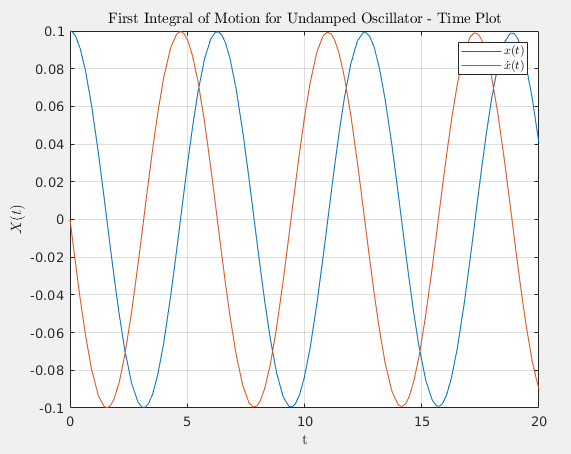
\includegraphics[width=.45\textwidth]{fig01.png}
  \centering
\end{figure}

c) Plot the vector field \(f(X)\) in the phase plane \((x_1, x_2)=(x, \dot{x})\). Plot for points spaced in a uniform mesh in the box \(x_1=[-10,10]\), \(x_2=[-10,10]\).
\begin{figure}[h]
  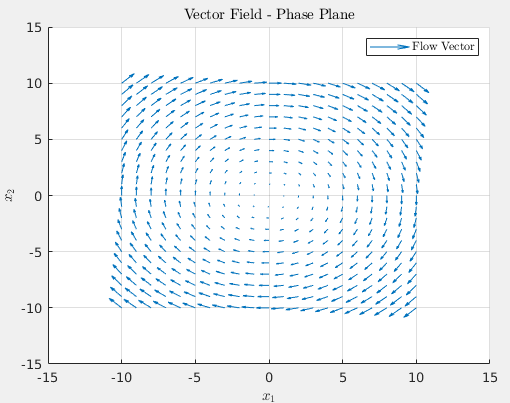
\includegraphics[width=.45\textwidth]{fig02.png}
  \centering
\end{figure}

d) Plot the system trajectories (flows or orbits) in the phase plane. Take ICs spaced in a uniform mesh in the box \(x_1=[-10,10]\), \(x_2=[-10,10]\).
\begin{figure}[h]
  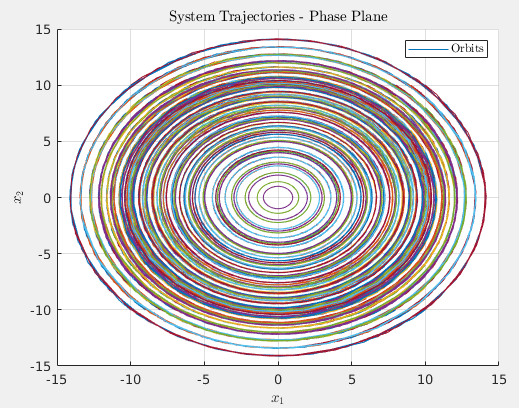
\includegraphics[width=.45\textwidth]{fig03.png}
  \centering
\end{figure}
\newpage
e) Derive the First Integral of Motion \(F(x_1,x_2)\) as done in class. Plot the FIM as a 3-D surface over the phase plane on the \(x_1=[-10,10]\), \(x_2=[-10,10]\).
\begin{equation*}
  \ddot{x} + x = 0 \Rightarrow \ddot{x} \textcolor{red}{\dot{x}} + x \textcolor{red}{\dot{x}} = 0 ~~;~~~~
\end{equation*}
Where
\begin{equation*}
  \frac{d}{dt}\left( \frac{1}{2} \dot{x}^2 +  \frac{1}{2} x^2 \right) = 0 \Rightarrow ~~~~ F(x) = \frac{1}{2} x_2^2 +  \frac{1}{2} x^2_1 ~~;~~~~
\end{equation*}
\begin{equation*}
\dot{F}(x) = \frac{\partial F}{\partial x} \dot{x}~~~;~~~~ \frac{\partial F}{\partial x} =
\begin{bmatrix}
  x_1 & x_2
\end{bmatrix}~~;~~~~
\dot{x} =
\begin{bmatrix}
  x_2 \\
  -x_1
\end{bmatrix}
\end{equation*}

Hence, we have FIM as
\begin{equation*}
  \dot{F}(x) =
  \begin{bmatrix}
    x_1 & x_2
  \end{bmatrix}
  \begin{bmatrix}
    x_2 \\
    -x_1
  \end{bmatrix}
  = 0
\end{equation*}
\begin{figure}[h]
  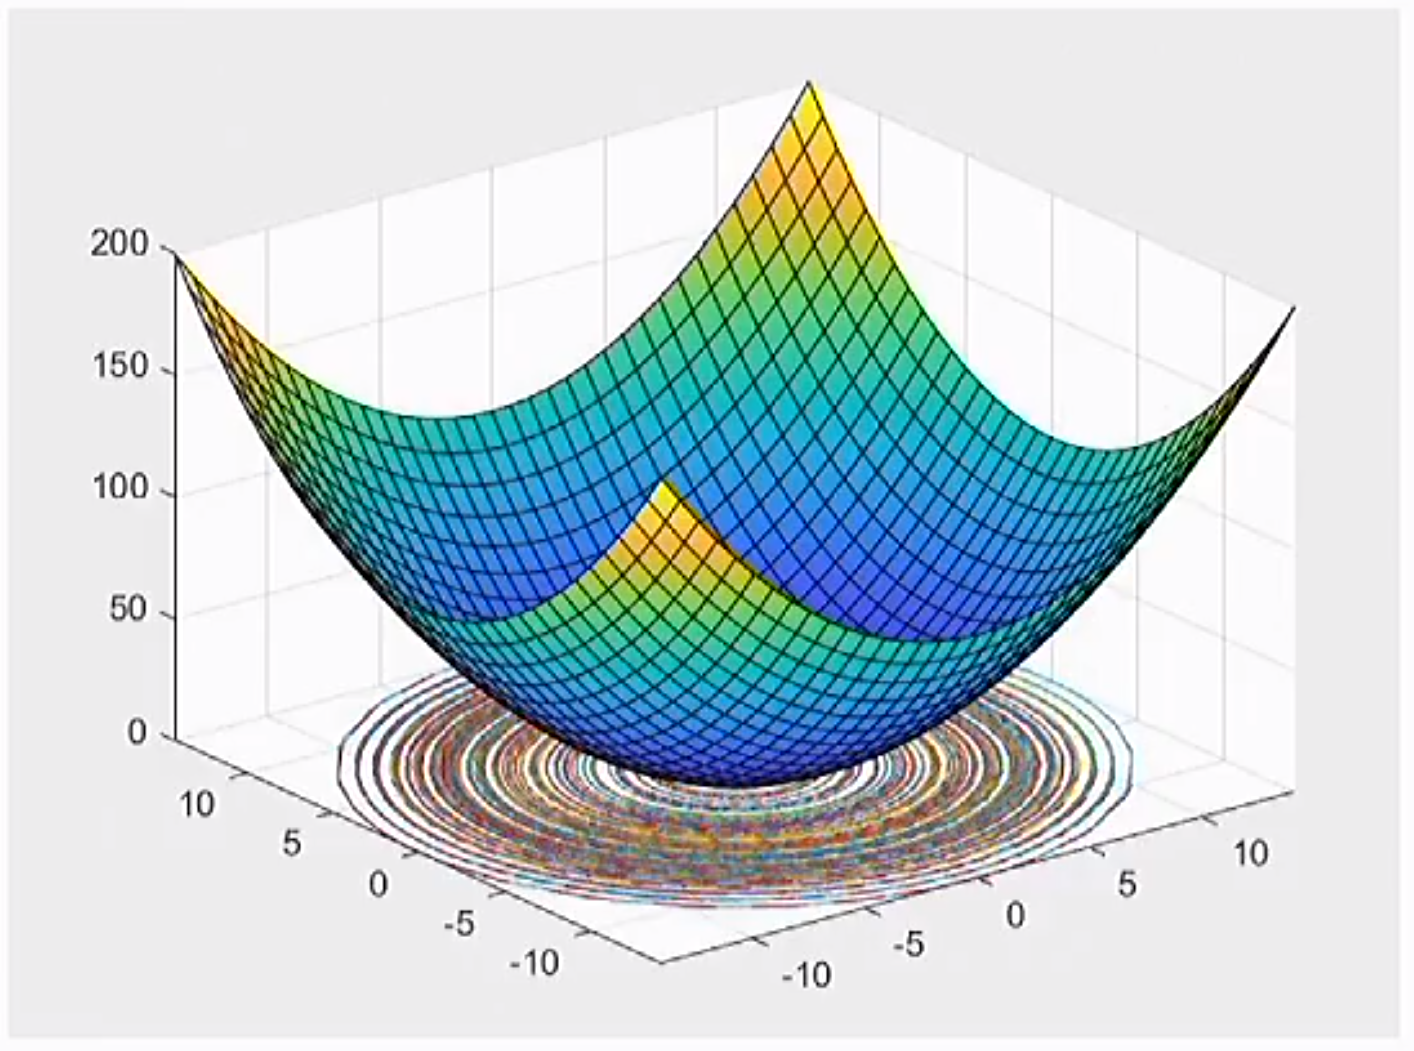
\includegraphics[width=.45\textwidth]{fig04.png}
  \centering
\end{figure}

\newpage
\noindent
\textbf{Matlab Code}\\
\lstinputlisting{hw04_q01_code.m}



\exercise
\noindent
\textbf{First Integral of Motion for Undamped Oscillator}\\
\begin{equation*}
\ddot{x} + x = 0
\end{equation*}

\begin{enumerate}[label=(\alph*)]
  \item Write position-velocity state space form \(\dot{X} = f(X)\).
  \item Plot the trajectories \(x(t)\), \(\dot{x}(t)\) vs. time. Use initial conditions of \(x(0)=0.1\), \(\dot{x}(t)=0\).
  \item Plot the vector field \(f(X)\) in the phase plane \((x_1, x_2)=(x, \dot{x})\). Plot for points spaced in a uniform mesh in the box \(x_1=[-10,10]\), \(x_2=[-10,10]\).
  \item Plot the system trajectories (flows or orbits) in the phase plane. Take ICs spaced in a uniform mesh in the box \(x_1=[-10,10]\), \(x_2=[-10,10]\).
  \item Derive the First Integral of Motion \(F(x_1,x_2)\) as done in class. Plot the FIM as a 3-D surface over the phase plane on the \(x_1=[-10,10]\), \(x_2=[-10,10]\).
\end{enumerate}


\noindent
\textbf{Answer} \\
a) Write position-velocity state space form \(\dot{X} = f(X)\).
\begin{equation*}
  \ddot{x} - x = 0 \Rightarrow \ddot{x} = +x \Rightarrow
\end{equation*}
\begin{equation*}
  X =
  \begin{bmatrix}
    x \\
    \dot{x}
  \end{bmatrix}
  = \begin{bmatrix}
    x_1 \\
    x_2
  \end{bmatrix} ~;~~ \dot{X} =
  \begin{bmatrix}
    x_2 \\
    x_1
  \end{bmatrix} = f(x)
\end{equation*}
State space form:
\begin{equation*}
  \dot{X} = AX \Rightarrow
  \begin{bmatrix}
    \dot{x} \\
    \ddot{x}
  \end{bmatrix} =
  \begin{bmatrix}
    0 & 1 \\
    1 & 0
  \end{bmatrix}
  \begin{bmatrix}
    x \\
    \dot{x}
  \end{bmatrix}
\end{equation*}

\newpage
b) Plot the trajectories \(x(t)\), \(\dot{x}(t)\) vs. time. Use initial conditions of \(x(0)=0.1\), \(\dot{x}(t)=0\).
\begin{figure}[h]
  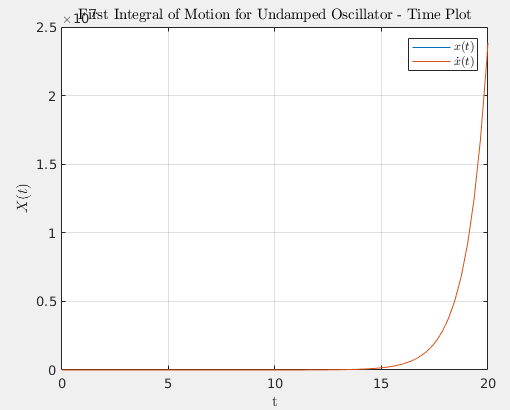
\includegraphics[width=.45\textwidth]{fig05.png}
  \centering
\end{figure}

c) Plot the vector field \(f(X)\) in the phase plane \((x_1, x_2)=(x, \dot{x})\). Plot for points spaced in a uniform mesh in the box \(x_1=[-10,10]\), \(x_2=[-10,10]\).
\begin{figure}[h]
  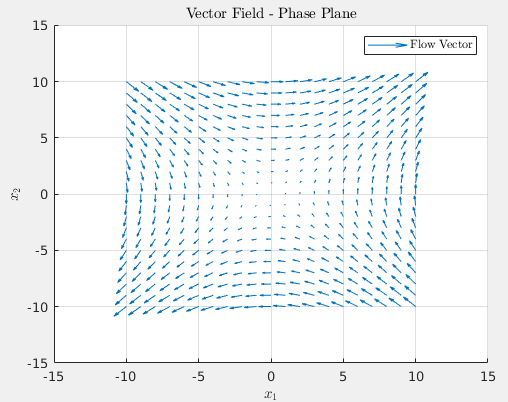
\includegraphics[width=.45\textwidth]{fig06.png}
  \centering
\end{figure}

d) Plot the system trajectories (flows or orbits) in the phase plane. Take ICs spaced in a uniform mesh in the box \(x_1=[-10,10]\), \(x_2=[-10,10]\).
\begin{figure}[h]
  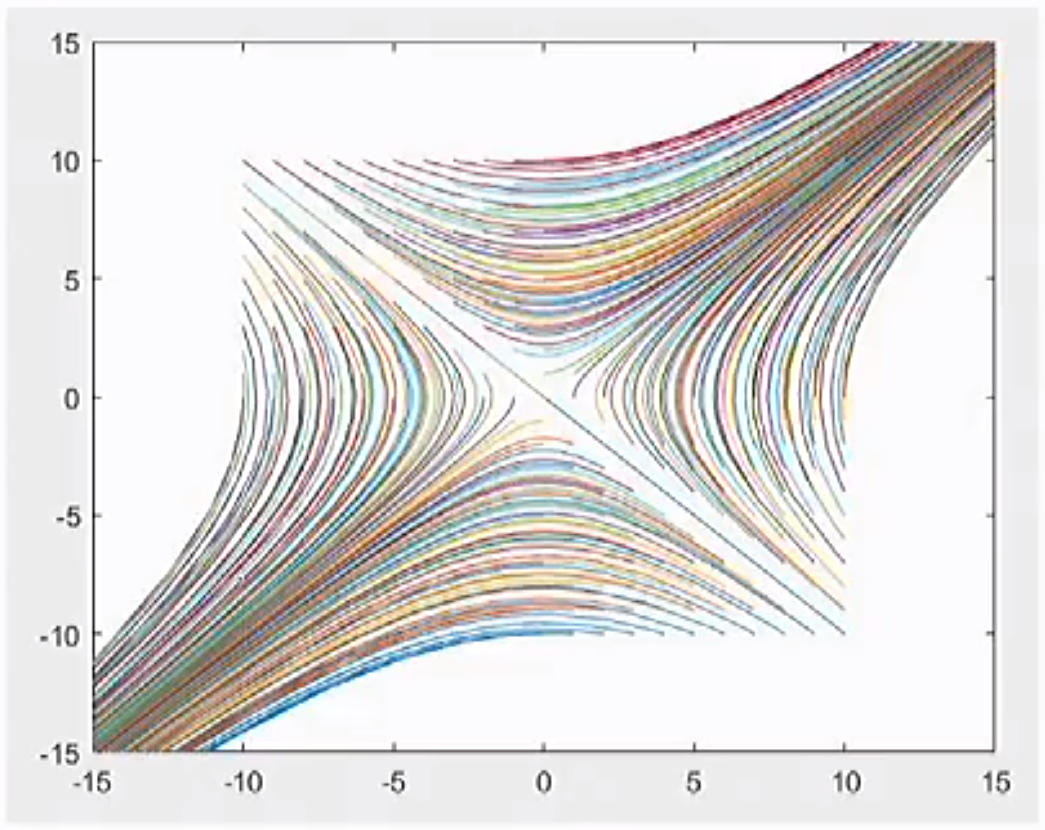
\includegraphics[width=.45\textwidth]{fig07.png}
  \centering
\end{figure}
\newpage
e) Derive the First Integral of Motion \(F(x_1,x_2)\) as done in class. Plot the FIM as a 3-D surface over the phase plane on the \(x_1=[-10,10]\), \(x_2=[-10,10]\).
\begin{equation*}
  \ddot{x} + x = 0 \Rightarrow \ddot{x} \textcolor{red}{\dot{x}} -x \textcolor{red}{\dot{x}} = 0 ~~;~~~~
\end{equation*}
Where
\begin{equation*}
  \frac{d}{dt}\left( -\frac{1}{2} \dot{x}^2 -  \frac{1}{2} x^2 \right) = 0 \Rightarrow ~~~~ F(x) =- \frac{1}{2} x_2^2 -  \frac{1}{2} x^2_1 ~~;~~~~
\end{equation*}
\begin{equation*}
\dot{F}(x) = \frac{\partial F}{\partial x} \dot{x}~~~;~~~~ \frac{\partial F}{\partial x} =
\begin{bmatrix}
  -x_1 & x_2
\end{bmatrix}~~;~~~~
\dot{x} =
\begin{bmatrix}
  x_2 \\
  x_1
\end{bmatrix}
\end{equation*}

Hence, we have FIM as
\begin{equation*}
  \dot{F}(x) =
  \begin{bmatrix}
    -x_1 & x_2
  \end{bmatrix}
  \begin{bmatrix}
    x_2 \\
    x_1
  \end{bmatrix}
  = 0
\end{equation*}
\begin{figure}[h]
  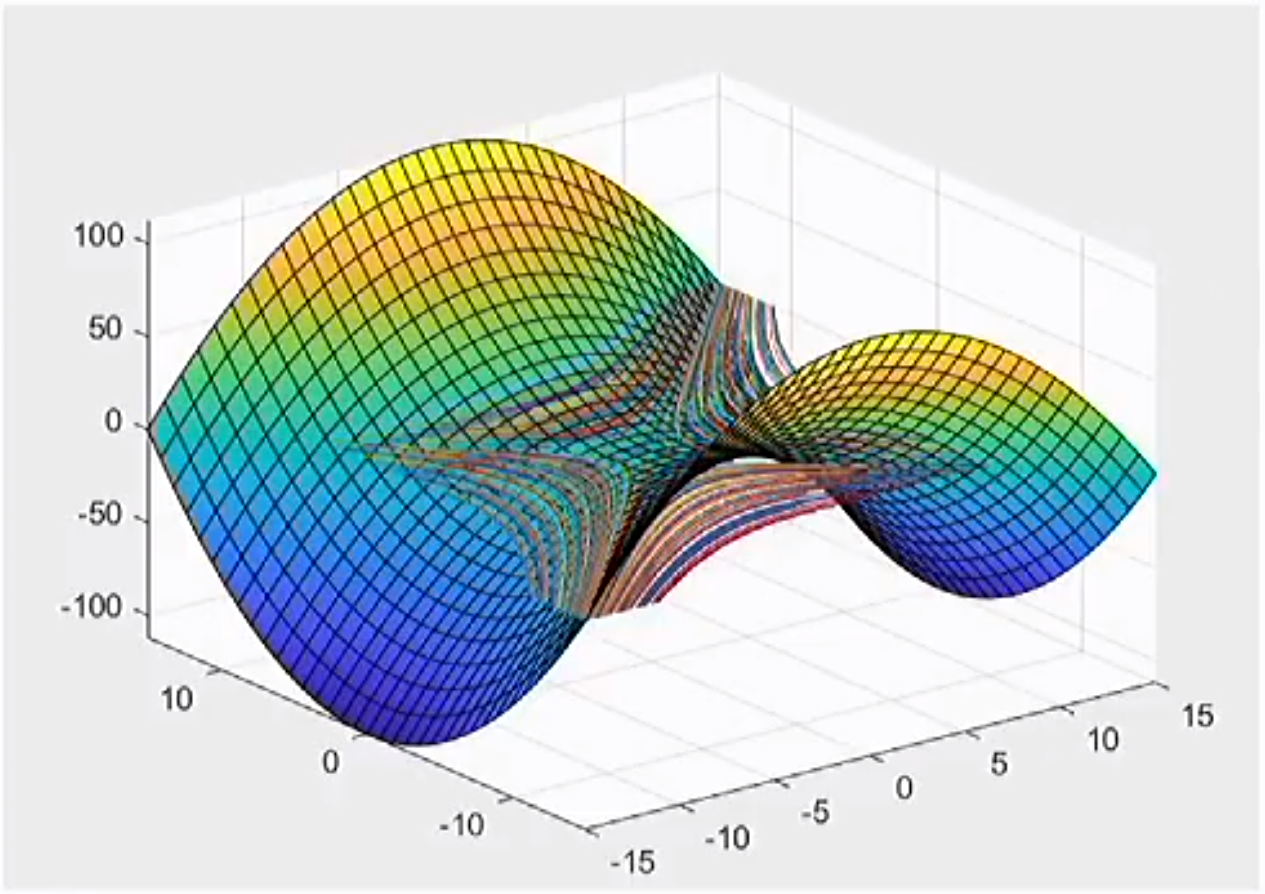
\includegraphics[width=.45\textwidth]{fig08.png}
  \centering
\end{figure}

\newpage
\noindent
\textbf{Matlab Code}\\
\lstinputlisting{hw04_q02_code.m}


%\bibliography{ref}

\end{document}
